\documentclass{beamer}

\usepackage[utf8]{inputenc}
\usepackage{amsfonts}
\usepackage{amsmath}
\usepackage{multicol}
\usepackage[noend]{algpseudocode}
\usefonttheme{serif}
\usetheme{Boadilla}
\usecolortheme{seahorse}


\title{Biomimicry of Bacterial Foraging}
\subtitle{for Distributed Optimization and Control}
\author{
  Kevin M. Passino\inst{1}\\
  Presented by: Alexander Van de Kleut\inst{2}
}
\institute{\inst{1}
  The Ohio State University\\
  Electrical and Computer Engineering
  \and
  \inst{2}
  University of Waterloo\\
  Centre for Theoretical Neuroscience
}
\date{IEEE Control Systems Magazine, 2002}

\begin{document}

\frame{\titlepage}

\begin{frame}
\frametitle{Table of Contents}
\tableofcontents
\end{frame}

% Kevin Passino is a professor of Electrical and Computer Engineering at Ohio State University.
% His work covers a broad range of disciplines, from virtual reality for mental health therapy to fuzzy control theory to humanitarian engineering.
% He has done considerable work on biomimicry and swarm intelligence.
% I've included here two selected textbooks he has been a major contributor for: Swarm Stability and Optimization, and Biomimicry for Optimization, Control, and Automation
% The paper I'm presenting today is Passino's second most-cited paper at over 3000 citations.
\section{About the Author}
\begin{frame}
\frametitle{About the Author}
\begin{columns}
  \column{0.5\textwidth}
    \includegraphics<1-2>[scale=2]{assets/kpassino}%
  \column{0.5\textwidth}
    \includegraphics<1>[scale=2]{assets/book1}
    \includegraphics<1>[scale=0.18]{assets/book2}
    \includegraphics<2>[scale=0.3]{assets/citations}
\end{columns}
\end{frame}

\section{Foraging}
\begin{frame}
\frametitle{Foraging}
\textbf{Foraging}
\begin{itemize}
  \item searching for nutrients
  \item avoiding noxious stimuli (toxins, predators, etc)
\end{itemize}
\textbf{Social Foraging}
\begin{itemize}
  \item increases likelihood of finding nutrients
  \item better detection and protection from noxious stimuli
  \item gains can offset cost of food competition
\end{itemize}
\end{frame}

\begin{frame}
\frametitle{Foraging as Optimization}
\textbf{How can we view foraging as an Optimization Process?}
\begin{itemize}
  \item<1-> We have some parameters $\theta$ and a loss function $J(\theta)$ that we want to minimize
  \item<2-> $\theta$ can represent the position of an organism in its environment
  \item<3-> $J$ can represent the concentration of nutrients and noxious stimuli
  \begin{itemize}
    \item smaller values of $J$ = more nutrients, less noxious stimuli
    \item higher values of $J$ = more noxious stimuli, less nutrients
  \end{itemize}
  \item<4-> In general, $J$ and $\theta$ can be arbitrary
  \begin{itemize}
    \item $\theta \in \mathbb{R}^p$
    \item $J: \mathbb{R}^p \to \mathbb{R}$
  \end{itemize}
\end{itemize}
\end{frame}

\section{Biological and Computational Model}
\begin{frame}
\frametitle{E. coli}
\begin{itemize}
  \item<1-> Model organism
  \begin{itemize}
    \item<2-> Highly studied
    \item<3-> Well-characterized foraging behaviour
    \item<4-> Probably won't feel bad about simplifying its behaviour
  \end{itemize}
  \item<5-> Social organism
  \begin{itemize}
    \item<6-> Secretes signals to attract others nearby
    \item<7-> Encourages ``swarming'' or ``clumping''
  \end{itemize}
\end{itemize}
\end{frame}

\begin{frame}
\frametitle{E. Coli Behaviour}
\begin{itemize}
  \item Swims using left-handed helical flagella (``propellers'')
  \begin{itemize}
    \item \textbf{Tumble}: flagella all rotate clockwise $\to$ pull on cell in all directions $\to$ random movement
    \item \textbf{Run}: flagella all rotate counterclockwise $\to$ flagella form a bundle $\to$ push on cell in one direction $\to$ directed movement
  \end{itemize}
\end{itemize}
\begin{center}
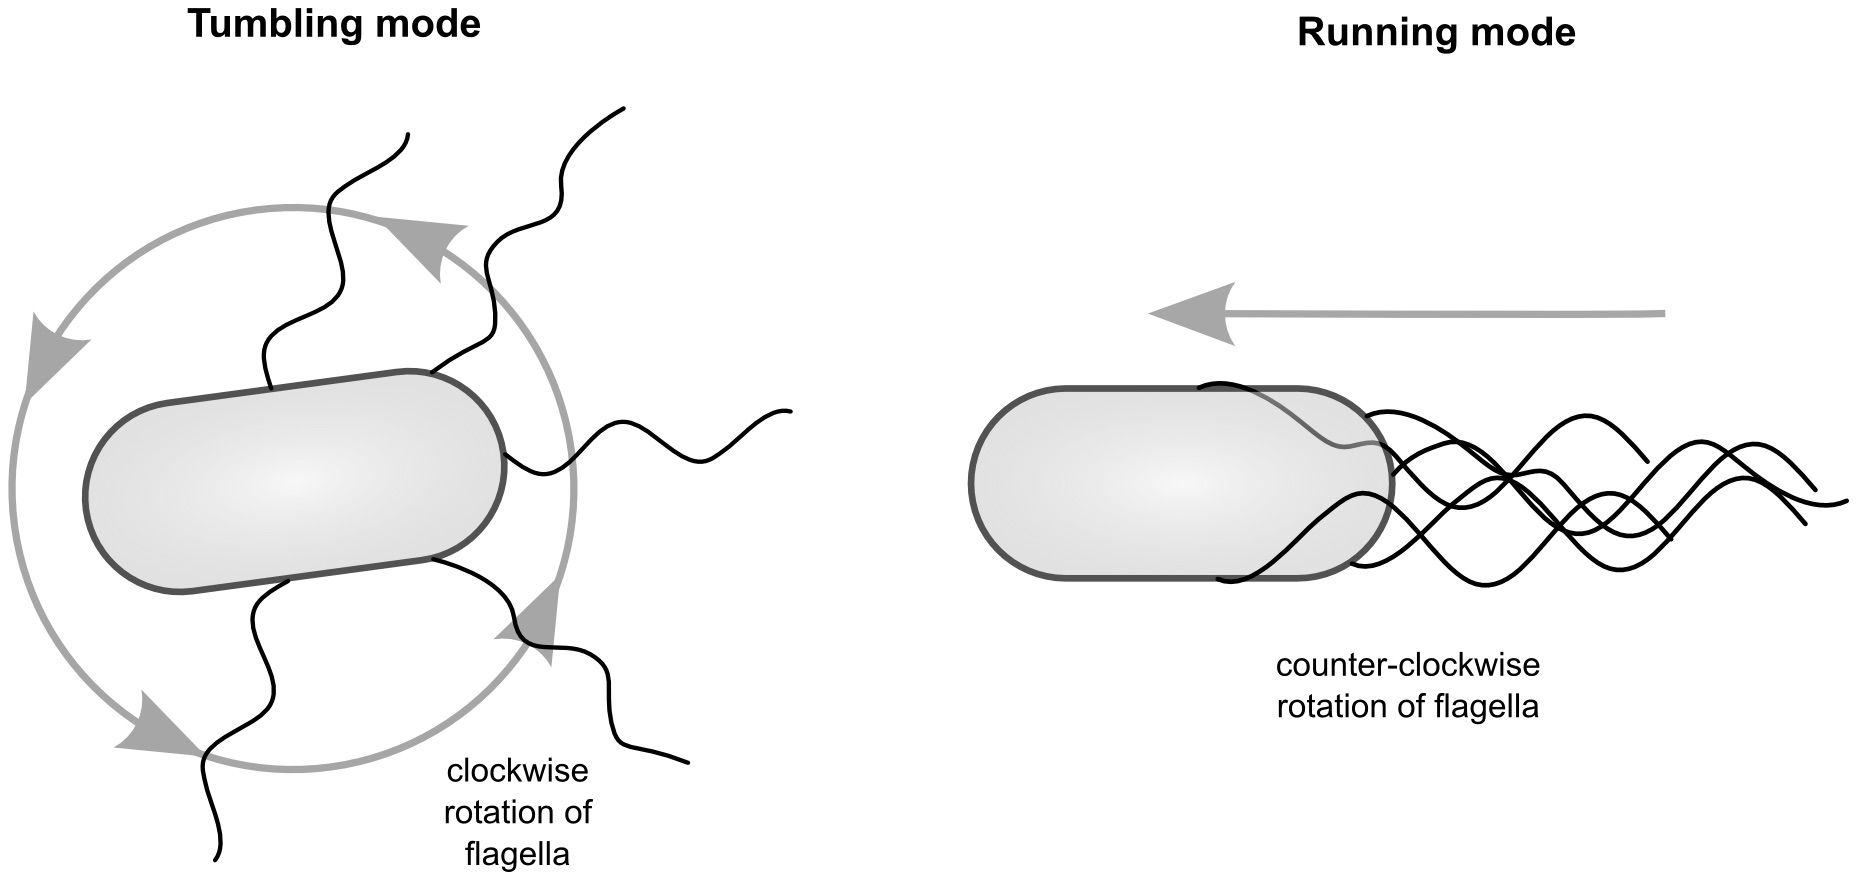
\includegraphics[scale=0.2]{assets/ecoli}
\end{center}
\end{frame}

\begin{frame}
\frametitle{E. Coli Behaviour}
\begin{itemize}
  \item If during a tumble E. Coli swims down a nutrient concentration gradient:
  \begin{itemize}
    \item Prolongs time spent on a run
    \item Continues moving in the same direction
  \end{itemize}
  \item Otherwise:
  \begin{itemize}
    \item Tends to switch to a tumble (search for more)
    \item Moves randomly which searching for more nutrient gradients to exploit
  \end{itemize}
\end{itemize}
\end{frame}

\begin{frame}
\frametitle{Algorithm for a Single Bacterium}
% \begin{multicols}{2}
\begin{algorithmic}[1]
\State $\theta \sim \mathcal{U}^p(\text{min}, \text{max})$
\For {$j \gets 1 \dots N_c $}:
  \State $\Delta \sim \mathcal{U}^p(-1, 1)$
  \State $J_\text{last} \gets J(\theta)$
  \State $\theta \gets \theta + C \frac{\Delta}{\| \Delta \|}$
  \For {$m \gets 1 \dots N_s$}:
    \If {$J(\theta) < J_\text{last}$}:
      \State $J_\text{last} \gets J(\theta)$
      \State $\theta \gets \theta + C \frac{\Delta}{\| \Delta \|}$
    \Else
      \State $m \gets N_s$
    \EndIf
  \EndFor
\EndFor
\end{algorithmic}
% \end{multicols}
\end{frame}

\begin{frame}
\frametitle{Algorithm for a Colony}
\begin{algorithmic}[1]
\For {$i \gets 1 \dots S$}:
  \State $\theta_i \sim \mathcal{U}^p(\text{min}, \text{max})$
\EndFor
\For {$j \gets 1 \dots N_c $}:
  \For {$i \gets 1 \dots S$}:
    \State $\Delta_i \sim \mathcal{U}^p(-1, 1)$
    \State $J_\text{last} \gets J(\theta_i)$
    \State $\theta_i \gets \theta_i + C \frac{\Delta_i}{\| \Delta_i \|}$
    \For {$m \gets 1 \dots N_s$}:
      \If {$J(\theta_i) < J_\text{last}$}:
        \State $J_\text{last} \gets J(\theta_i)$
        \State $\theta_i \gets \theta_i + C \frac{\Delta_i}{\| \Delta_i \|}$
      \Else
        \State $m \gets N_s$
      \EndIf
    \EndFor
  \EndFor
\EndFor
\end{algorithmic}
\end{frame}

\begin{frame}
\frametitle{E. Coli Swarming}

\end{frame}

\begin{frame}
\frametitle{Algorithm for a Colony with Swarming}
\begin{algorithmic}[1]
\For {$i \gets 1 \dots S$}:
  \State $\theta_i \sim \mathcal{U}^p(\text{min}, \text{max})$
\EndFor
\For {$j \gets 1 \dots N_c $}:
  \For {$i \gets 1 \dots S$}:
    \State $\Delta_i \sim \mathcal{U}^p(-1, 1)$
    \State $J_\text{last} \gets J(\theta_i) + J_{cc}(\theta_i)$
    \State $\theta_i \gets \theta_i + C(i) \frac{\Delta_i}{\| \Delta_i \|}$
    \For {$m \gets 1 \dots N_s$}:
      \If {$J(\theta_i) < J_\text{last}$}:
        \State $J_\text{last} \gets J(\theta_i) + J_{cc}(\theta_i)$
        \State $\theta_i \gets \theta_i + C(i) \frac{\Delta_i}{\| \Delta_i \|}$
      \Else
        \State $m \gets N_s$
      \EndIf
    \EndFor
  \EndFor
\EndFor
\end{algorithmic}
\end{frame}



% cons
% no attempts to compare to actual biological
% spends long time in introduction describing things like search strategies (cruise, ambush, saltatory), but only ends up using one
% discusses how foraging and looking for nutrients depends on the concentration of nutrients and how the nutrients can be used up, but then ignores this information when desigining the simulation
% do you want a gradient-free hill-climbing algorithm or a simulation of e coli behaviour?
%

\end{document}
